%  LaTeX support: latex@mdpi.com
%  In case you need support, please attach all files that are necessary for compiling as well as the log file, and specify the details of your LaTeX setup (which operating system and LaTeX version / tools you are using).

% You need to save the "mdpi.cls" and "mdpi.bst" files into the same folder as this template file.

%=================================================================
\documentclass[ijgi,article,submit,moreauthors,pdftex,10pt,a4paper]{mdpi} 

%--------------------
% Class Options:
%--------------------
% journal
%----------
% Choose between the following MDPI journals:
% actuators, admsci, aerospace, agriculture, agronomy, algorithms, animals, antibiotics, antibodies, antioxidants, applsci, arts, atmosphere, atoms, axioms, batteries, behavsci, beverages, bioengineering, biology, biomedicines, biomimetics, biomolecules, biosensors, brainsci, buildings, carbon, cancers, catalysts, cells, challenges, chemosensors, children, chromatography, climate, coatings, computation, computers, condensedmatter, cosmetics, cryptography, crystals, data, dentistry, designs, diagnostics, diseases, diversity, econometrics, economies, education, electronics, energies, entropy, environments, epigenomes, fermentation, fibers, fishes, fluids, foods, forests, futureinternet, galaxies, games, gels, genealogy, genes, geosciences, geriatrics, healthcare, horticulturae, humanities, hydrology, informatics, information, infrastructures, inorganics, insects, instruments, ijerph, ijfs, ijms, ijgi, inventions, jcdd, jcm, jdb, jfb, jfmk, jimaging, jof, jintelligence, jlpea, jmse, jpm, jrfm, jsan, land, languages, laws, life, literature, lubricants, machines, magnetochemistry, marinedrugs, materials, mathematics, mca, mti, medsci, medicines, membranes, metabolites, metals, microarrays, micromachines, microorganisms, minerals, molbank, molecules, mps, nanomaterials, ncrna, neonatalscreening, nutrients, particles, pathogens, pharmaceuticals, pharmaceutics, pharmacy, philosophies, photonics, plants, polymers, processes, proteomes, publications, recycling, religions, remotesensing, resources, risks, robotics, safety, sensors, separations, sexes, sinusitis, socsci, societies, soils, sports, standards, sustainability, symmetry, systems, technologies, toxics, toxins, universe, urbansci, vaccines, vetsci, viruses, water
%---------
% article
%---------
% The default type of manuscript is article, but can be replaced by: 
% addendum, article, book, bookreview, briefreport, casereport, changes, comment, commentary, communication, conceptpaper, correction, conferencereport, expressionofconcern, meetingreport, creative, datadescriptor, discussion, editorial, essay, erratum, hypothesis, interestingimage, letter, newbookreceived, opinion, obituary, projectreport, reply, retraction, review, sciprints, shortnote, supfile, technicalnote
% supfile = supplementary materials
%----------
% submit
%----------
% The class option "submit" will be changed to "accept" by the Editorial Office when the paper is accepted. This will only make changes to the frontpage (e.g. the logo of the journal will get visible), the headings, and the copyright information. Also, line numbering will be removed. Journal info and pagination for accepted papers will also be assigned by the Editorial Office.
%------------------
% moreauthors
%------------------
% If there is only one author the class option oneauthor should be used. Otherwise use the class option moreauthors.
%---------
% pdftex
%---------
% The option pdftex is for use with pdfLaTeX. If eps figure are used, remove the option pdftex and use LaTeX and dvi2pdf.

%=================================================================
\firstpage{1} 
\makeatletter 
\setcounter{page}{\@firstpage} 
\makeatother 
\articlenumber{x}
\doinum{10.3390/------}
\pubvolume{xx}
\pubyear{2016}
\copyrightyear{2016}
\externaleditor{Academic Editor: name}
\history{Received: date; Accepted: date; Published: date}
%------------------------------------------------------------------
% The following line should be uncommented if the LaTeX file is uploaded to arXiv.org
%\pdfoutput=1

%=================================================================
% Add packages and commands here. The following packages are loaded in our class file: fontenc, calc, indentfirst, fancyhdr, graphicx, lastpage, ifthen, lineno, float, amsmath, setspace, enumitem, mathpazo, booktabs, titlesec, etoolbox, amsthm, hyphenat, natbib, hyperref, footmisc, geometry, caption, url, mdframed

%=================================================================
%% Please use the following mathematics environments:
 \theoremstyle{mdpi}
 \newcounter{thm}
 \setcounter{thm}{0}
 \newcounter{ex}
 \setcounter{ex}{0}
 \newcounter{re}
 \setcounter{re}{0}

 \newtheorem{Theorem}[thm]{Theorem}
 \newtheorem{Lemma}[thm]{Lemma}
 \newtheorem{Corollary}[thm]{Corollary}
 \newtheorem{Proposition}[thm]{Proposition}

 \theoremstyle{mdpidefinition}
 \newtheorem{Characterization}[thm]{Characterization}
 \newtheorem{Property}[thm]{Property}
 \newtheorem{Problem}[thm]{Problem}
 \newtheorem{Example}[ex]{Example}
 \newtheorem{ExamplesandDefinitions}[ex]{Examples and Definitions}
 \newtheorem{Remark}[re]{Remark}
 \newtheorem{Definition}[thm]{Definition}
%% For proofs, please use the proof environment (the amsthm package is loaded by the MDPI class).

%=================================================================
% Full title of the paper (Capitalized)
\Title{Exploring multi-scale spatiotemporal Twitter user mobility patterns with a scalable visual-analytics framework}

% Authors, for the paper (add full first names)
\Author{Junjun Yin $^{1}$ and Zhenhong Du $^{2}$*}
% Authors, for metadata in PDF
\AuthorNames{Firstname Lastname, Firstname Lastname and Firstname Lastname}

% Affiliations / Addresses (Add [1] after \address if there is only one affiliation.)
\address{%
$^{1}$ \quad Department of Geography and Geographic Information Science, University of Illinois at Urbana-Champaign, Urbana, IL 61801, USA ; jyn@illinois.edu\\
$^{2}$ \quad Key Laboratory of Geographic Information Science, School of Earth Sciences, Zhejiang University, Hangzhou, 310028, China; duzhenhong@zju.edu.cn}

% Contact information of the corresponding author
\corres{Correspondence: duzhenhong@zju.edu.cn; Tel.: +8613819192989}

% Current address and/or shared authorship

% Simple summary
%\simplesumm{}

% Abstract (Do not use inserted blank lines, i.e. \\) 
\abstract{Understanding human mobility patterns is of great importance for urban planning, traffic management, and even marketing campaign.
However, the capability of capturing detailed human movements with fine-grained spatial and temporal granularity is still limited.
In this study, we have extracted high-resolution mobility data from a collection of 1.3 billion geo-located Twitter messages to study multi-scale spatiotemporal Twitter user mobility patterns in the United States during the year 2014. 
Regarding the concerns of infringement on individual privacy, such as the mobile phone call data with restricted access, the dataset is collected from publicly accessible Twitter data streams.
In this study, we have developed a scalable visual-analytics framework to deliver efficiency and scalability in filtering large volume of geo-located tweets, modeling and extracting Twitter user movements, generating space-time user trajectories, and summarizing multi-scale spatiotemporal user mobility patterns.
We have performed a set of statistical analysis to understand Twitter user mobility patterns across multi-level spatial scales and temporal granularity.
In particular, the Twitter user mobility patterns measured by the displacements and radius of gyrations of individuals have revealed multi-scale or multi-modal Twitter user mobility patterns.
By further studying such mobility patterns in different temporal ranges, we have identified both consistency and seasonal fluctuations regarding the distance decay effects in the corresponding mobility patterns.}

% Keywords
\keyword{Geo-located tweets, mobility patterns, multi-scale spatiotemporal analysis, scalable visual-analytics framework}
\begin{document}

%%%%%%%%%%%%%%%%%%%%%%%%%%%%%%%%%%%%%%%%%%
%% Sections that are not mandatory are listed as such. The section titles given are for Articles. Review papers and other article types have a more flexible structure. 

%% Only for the journal Gels: Please place the Experimental Section after the Conclusions

%%%%%%%%%%%%%%%%%%%%%%%%%%%%%%%%%%%%%%%%%%
\section{Introduction}
Understanding human mobility patterns is of great importance for a broad range of applications from urban planning~\cite{zheng2008understanding}, traffic management~\cite{jiang2009characterizing}, and even the spatial spread of epidemic diseases~\citep{belik2011natural}.
Earlier research efforts relied on low resolution mobility data to understand human mobility patterns, such as using census records to understand human migration patterns~\citep{greenwood1985human}, or delivering questionnaires and asking volunteers to report the track of bank notes to infer human travel patterns~\citep{brockmann2006scaling}.
However, the lack of detailed human movements with fine-grained spatial and temporal granularity limits the findings to capture mobility patterns of individuals~\citep{gonzalez2008understanding,Jurdak2015}.
In addition to the mobility data collected by GPS trackers~\citep{zheng2008understanding, rhee2011levy} and mobile phone call records~\citep{gonzalez2008understanding,sevtsuk2010does,kung2014exploring}, 
emerging as a new source for mobility data, today's pervasive Location Based Social Media (LBSM) platforms (e.g., Twitter and Foursquare) offer continuous spatial Big Data streams with massive amount of detailed and frequently updated user digital footprints~\citep{thatcher2014living} in the form of real-world trails and footprints.
One significant advantage of LBSM data streams is the large spatial coverage, for example, researchers have used geo-located Twitter data for studying global mobility patterns~\citep{hawelka2014geo}, which is otherwise impossible by using other mobility datasets (e.g., GPS traces and mobile phone call records). 
In addition, the publicly available LBSM data streams offer unique opportunities for conducting replicable scientific findings regarding the concerns of infringement on individual privacy, such as using mobile phone call records~\citep{giannotti2008mobility,crampton2014collect,Jurdak2015}.

Many studies have adopted the LBSM data streams to study human mobility patterns. For example, they modeled and extracted trajectories of individuals and performed statistical analysis focusing on the distance decay effects~\citep{gonzalez2008understanding} in the collective user movements to reveal different travel modes~\citep{Jurdak2015}, travel demands~\citep{wu2014intra,hasan2013understanding}, and the impact of social connections~\citep{cho2011friendship}.
These studies have provided strong support for using LBSM data as proxies for studying mobility patterns of individuals and valuable insights into human mobility dynamics. 
However, in these studies, the measurements of distances are either fixed in a certain time period or a specific region, where they do not consider the variations of movements in different spatial scales and temporal ranges.
To be more specific, these studies lack examinations of the detailed movements across different geographical scales and temporal granularity, for instances, whether there are temporal (e.g., monthly or seasonal) changes within the movements, and how the mobility patterns vary across different spatial scales (e.g., intra- or inter county, city or country level). 
These insights are critical to advance our understandings of the collective mobility patterns for a variety of applications, such as examining the mobility patterns across different cities~\citep{noulas2012tale}, the spread patterns of disease~\citep{balcan2009multiscale, tamerius2011global} and touristic activities~\citep{hawelka2014geo}.
While the high resolution spatiotemporal records from LBSM present unique research opportunities in this direction, the inherited large data volume poses significant data intensive challenges for developing a multi-scale spatiotemporal analysis framework~\citep{tsou2015} to deal with the complexities in filtering movements of individuals, modeling and aggregating user trajectories at multiple spatial and temporal scales.
In addition, to enable efficient analysis and visualization of the mobility patterns at different spatiotemporal scales, it is essential for such a framework to provide scalability for addressing the data intensive challenges~\citep{cao2014scalable}. 

In this paper, we have explored and studied the Twitter user mobility patterns across multi-level spatial scales and temporal granularity in the United States during the year 2014. 
The mobility data is extracted from1.3 billion geo-located Twitter messages (i.e., tweets) from 1$^{st}$ January to 31$^{st}$ December, 2014 in the United States with over 6 million Twitter users and over 1 TB in file size. 
To address the data-intensive challenges embedded in this dataset, we have developed a scalable visual-analytics framework tailored to accommodate large volume of geo-located tweets for studying multi-level spatiotemporal Twitter user mobility patterns.
This framework is implemented based on high-performance distributed computing environment using Apache Hadoop\footnote{http://hadoop.apache.org/}, which is an open source software framework to enable distributed processing of large datasets across computing clusters.
%We have implemented a set of efficient MapReduce~\citep{dean2008mapreduce} algorithms to deliver scalability in filtering large volume of geo-located tweets, modeling and extracting Twitter user movements, generating space-time user trajectories, and summarizing multi-level spatiotemporal user mobility patterns.
With this framework, we have performed a set of statistical analysis to understand the spatiotemporal Twitter user mobility patterns. 
We have modeled the frequency of Twitter users visiting different locations to study the collective user visiting behaviors, where we have identified temporal similarities in the distributions. 
In particular, the Twitter user mobility patterns measured by the displacements and radius of gyrations of individuals~\citep{gonzalez2008understanding} have revealed different groups of Twitter users with multi-scale or multi-modal mobility patterns and multiple travel modes~\citep{Jurdak2015}.
By further studying such mobility patterns in different temporal ranges, we have identified both consistency and seasonal fluctuations regarding the distance decay effects in the corresponding mobility patterns. 

The remainder of this paper is organized as follows.
Section 2 describes the related work in the context of studying mobility patterns using LBSM data, in particular, geo-located Twitter data.
We focus on research challenges in visual-analytics methods to enable multi-scale
spatiotemporal analysis with massive movement datasets, including data management, multi-level spatiotemporal user trajectory modeling and visualization.
Section 3 details the processes for extracting, aggregating and summarizing multi-level spatiotemporal Twitter user mobility patterns.
Section 4 presents the case study of performing visual-analytics for seeking Twitter mobility patterns in the United States of year 2014. Section 5 concludes the paper.

\section{Mobility patterns in Location Based Social Media data}
\subsection{Geo-located Twitter data for studying large-scale user movements}
To understand detailed human mobility patterns of individuals, the capability of capturing human movements with fine-grained spatial and temporal granularity is critical.
However, the low-resolution mobility data collected from census records~\citep{greenwood1985human} is estimated and aggregated at census tract level, while tracking of bank notes~\citep{brockmann2006scaling} is at zip code level and do not necessarily reflecting movements of the same individuals~\citep{gonzalez2008understanding}.
In terms of collecting detailed mobility data of individuals, using GPS trackers tends to produce, to date, the most accurate records of individuals' movements regarding the accuracy of recorded user locations and update frequency~\citep{zheng2008understanding}. However, the data is often limited in spatial scale (e.g. within a specific city or region) with a small group of people, for example, 182 and 226 volunteers participated in collecting such mobility data in~\citep{zheng2010geolife} and~\citep{rhee2011levy} respectively. Other than tracking people directly, the vehicle-based GPS data is often tied to a specific vehicle (e.g. taxi), which may only be accessible for a certain group of people~\citep{kung2014exploring}. 

Another approach from the literatures for studying human mobility is using mobile phone call data in the form of Call Detail Records (CDR), where the locations of mobile users are estimated by cell tower triangulation with accuracy in the order of kilometers~\citep{gonzalez2008understanding,sevtsuk2010does,kung2014exploring}. 
Such a dataset can cover relatively large spatial scale (e.g., country level)~\citep{becker2013human,sobolevsky2013delineating} and a large portion of the population in the study region~\citep{kung2014exploring}. However, due to the concerns of infringement on individual privacy, the mobile phone call data is not publicly accessible, which is not ideal  for conducting replicable scientific findings, such as validating or extending the existing discoveries.

In this connection, it becomes increasingly popular for researchers to exploit the publicly accessible mobility data captured from today's pervasive Location Based Social Media (LBSM) platforms (e.g., Foursquare and Twitter). 
LBSM enables users to attach their current location as a geo-tag to the message they will post, which is derived from either the GPS or Wi-Fi positioning with a high position resolution down to 10 meters~\citep{Jurdak2015}.
A Big Data scenario emerges when millions social media users constantly posting messages.
However, there are some limitations and complexities in directly using the LBSM data for study human mobility patterns. 
For example, comparing to GPS traces, the update frequency of an individual's location varies depending on when a user is posting a new geo-located message or check-in at a new place. It has been criticized for the lack of representativeness of the population as not all people use social media or send geo-located messages~\citep{kung2014exploring}. Another research challenge is to identify the users, as a social media account is not equal to a real person in the physical world~\citep{tsou2015}.
Although many studies started to look into the demographic information of LBSM data, in particular Twitter data~\citep{mitchell2013geography,longley2015geotemporal}, these issues certainly require us to pose more strict criteria in filtering and extracting individual movements.

In this study, geo-located Twitter data is chosen as source for studying detailed mobility patterns. Compared to other LBSM platforms, Twitter is one of the most popular platforms and is been actively used in many countries. It provides a publicly accessible streaming API\footnote{https://dev.twitter.com/streaming/overview} for easy access to its data, in fact, many other LBSM data can be collected from the data streams, such as Foursquare check-in data~\citep{cranshaw2012livehoods, hasan2013understanding}.
In addition, it presents some unique advantages that make it suitable for studying human mobility patterns.
For example, the high-resolution location information enables to identify multiple travel modes in user mobility patterns~\citep{Jurdak2015}; the large spatial coverage enables to study global mobility patterns~\citep{hawelka2014geo}, which is almost impossible for other mobility datasets.
More importantly, by continuously monitoring the geo-located Twitter data streams with large volumes of detailed and frequently updated spatiotemporal  records of Twitter users, it offers a great deal of potential for studying mobility patterns of large groups of individuals at different spatial scales (e.g., movements across cities, states or even countries) and temporal gratuity (e.g., weekly, monthly, and seasonal movements).

\subsection{Data-intensive challenges for multi-scale geo-visual analytics}
Mobility data is essentially a collection of spatiotemporal records of people moving from one location to another in the geographic space.
To study mobility patterns of individuals, a space-time trajectory of each individual should be modeled and constructed to quantify the collective movements over space and time.
Based on the extracted space-time trajectories, aforementioned studies are able to perform analysis, such as the measurements of displacements and radius of gyrations of individuals, to study the mobility dynamics.
At the same time, space-time trajectory is one of the core concepts in H{\"a}gerstrand's time geography to understand the embedded spatiotemporal dynamics~\citep{hagerstrand1985time}, which has provided useful insights to explore movements across different geographical scales and temporal granularity.
For example, a geo-visualization approach was used to study human activity patterns, where user trajectories are mapped in a 3D space ordered by timestamps in the third dimension~\citep{kwan2004geovisualization}. While such an approach enables visualization of detailed trajectories, its capability is limited in dealing with large-volume movement datasets~\citep{andrienko2007designing}.
Instead of directly visualizing individual user trajectories, a space-time cube approach was proposed in analyzing and visualizing the collective trajectories by providing flexibilities in setting up both spatial and temporal ranges, and therefore to study the mobility patterns across different spatial units (e.g. countries, states, and cities, etc.) and identify the changes over space and time~\citep{maceachren2001research, maceachren2004maps}.
In this connection, visual-analytics methods are proposed to help better convey the findings in terms of analyzing and visualizing multi-level spatiotemporal mobility patterns~\citep{andrienko2007designing,andrienko2007visual}.
Visual-analytics methods focus on the synergy of computational and analytical methods to reduce the visual clutter, where aggregation methods are suggested to perform grouping/dividing individual's moving trajectories at different spatial and temporal granularity, e.g., utilizing the space-time cube approach~\citep{andrienko2007designing}.

Employing visual-analytics methods dealing with massive movement datasets is not only beneficial for optimizing visualizations but also provides a great deal of flexibilities for performing statistical analysis in seeking mobility patterns with different level of spatiotemporal details. 
By conveying the findings from statistical analysis, it provides another visualization form regarding the corresponding mobility patterns, in a sense, to avoid the problems of visual clutters.
However, in the context of studying mobility patterns using large volume of geo-located Twitter data, the inherited large data volume poses significant data intensive challenges for these mentioned visual-analytics methods to scale with both the data volume and the computational requirements (e.g., movement extraction and trajectory modeling)~\citep{cao2014scalable}.
For example, in our study, 1.3 billion geo-located tweets were collected with over 1 TB in file size.
To construct a space-time trajectory of an individual, it is necessary to go through the massive dataset to sort and update the trajectory whenever a new location is found. 
Such a task is already computationally demanding, let along breaking the trajectories to construct space-time cube with multiple spatial scale and temporal ranges. 
In particular, developing a multi-scale spatiotemporal analysis framework is identified as one of the research challenges for dealing with social media Big Data~\citep{tsou2015}. 
To address the data-intensive challenges, there is a need to develop a scalable visual-analytics framework tailored to accommodate large volume of geo-located tweets for studying multi-level spatiotemporal Twitter user mobility patterns.

%\subsection{Accommodating LBSM Big Data with Hadoop}
%Apache Hadoop is an open source software framework designed to facilitate data intensive computing on large commodity clusters.
%It combines a distributed file system, namely Hadoop Distributed File System(HDFS)~\citep{shvachko2010hadoop} with MapReduce programming paradigm, which can be applied to wide range of data-intensive problems.
%MapReduce is a programming model and an associated software framework designed to process massive data in a distributed fashion~\citep{dean2008mapreduce}.
%MapReduce breaks the entire computation into small tasks and schedule them among different computing nodes.
%MapReduce consists of two main stages: map and reduce.
%In the map stage, input data is converted into series of intermediate $\langle key, value\rangle$ pairs.
%Customized computation will be performed in the reduce stage based on the same intermediate key.
%This framework provides parallelization since both map and reduce tasks are considered independent and can be done in parallel. More importantly, it provides scalability in relation to the growth of data size, where Hadoop can scale to more computing nodes in the cluster to maintain the performance.
%
%Our framework benefits from using Hadoop in both data management and processing.
%First, since the input data is large it is desirable to store it on multiple machines.
%Second, by using Hadoop we can parallelize the computational tasks and make the data processing faster and more efficient.
%Further, by adopting the MapReduce computing paradigm, we can model each individual user's trajectory by treating user's unique ID as key, and summarize the movement flows among different spatial units by utilizing the ID of the spatial unit as key. The details will be introduced in the following section.

\section{Materials and Methods}
\subsection{Geo-located Twitter data}
Geo-located tweets are tweets appended with an additional geo-tag in the form of a pair of geographical coordinates, which represents the location a tweet was sent at. 
In this study, the geo-located tweets were downloaded using the Twitter Streaming API, where we specified a geographical bounding box as an area-of-interest to retrieve all the geo-located tweets that fall within it. 
To ensure complete coverage over the United States, we implemented a crawler that selects North America as the initial area-of-interest, where the geographical boundary is specified with lower left (latitude: 5.4, longitude: -167.3) and upper right (latitude: 83.2, longitude: -52.2).
The crawler is constantly running with over 2 million geo-located raw tweets ($\sim$2GB in size) collected per day.
We have collected more than 1.3 billion geo-located tweets from 1$^{st}$ January to 31$^{st}$ December, 2014 with 6,147,430 Twitter users and 1 TB in file size.

As a social media account is not equal to a real person in the physical world~\citep{tsou2015}, to ensure the data quality, the collected raw tweets were further filtered by the following steps: We first removed the duplicated messages\footnote{https://support.twitter.com/articles/18311-the-twitter-rules} in the dataset; and then we attempted to remove non-human users based on unusual relocating speed (Hawelka et al., 2014; Jurdak et al., 2015). 
In this case, we adopted the speed limit value as 240 m/s used in (Jurdak et al., 2015), where we examined all the consecutive locations of each user and excluded those with relocating speed over the limit.
Note that the original location information embedded in each geo-located tweet is given in units of latitude and longitude. To reduce the complexity in calculating distances and performing spatial aggregations directly based on geographical coordinates, we projected the all the points using North America Albers Equal Area Conic (ESRI:102008) coordinate system.
Finally, we used the geographic boundaries of the United States\footnote{https://www.census.gov/geo/maps-data/data/} (excluding Alaska and Hawaii) to further restrict the remaining tweets, where the technical details is presented in the following section. Based on these reinforcements, the dataset contains 1,052,861,000 tweets and 4,559,205 unique users.

\subsection{A scalable visual-analytics framework}
To address the data-intensive challenges, we have developed a scalable visual-analytics framework tailored to accommodate large volume of geo-located tweets for studying multi-level spatiotemporal Twitter user mobility patterns.
The scalable visual-analytics framework consists of two main units: (1) Data collection unit: a Twitter data crawler that continuously collects raw geo-located tweets using the Twitter Streaming API. (2) Data processing unit: a distributed computing environment using Apache Hadoop for modeling and extracting Twitter user movements, generating space-time user trajectories, and summarizing the movements at multiple spatiotemproal levels.
An overall system architecture of the framework that chains the three units is shown in Figure 1. The details regarding the function and implementation of each unit are presented in the next sections.

\begin{figure}[h]
\centering
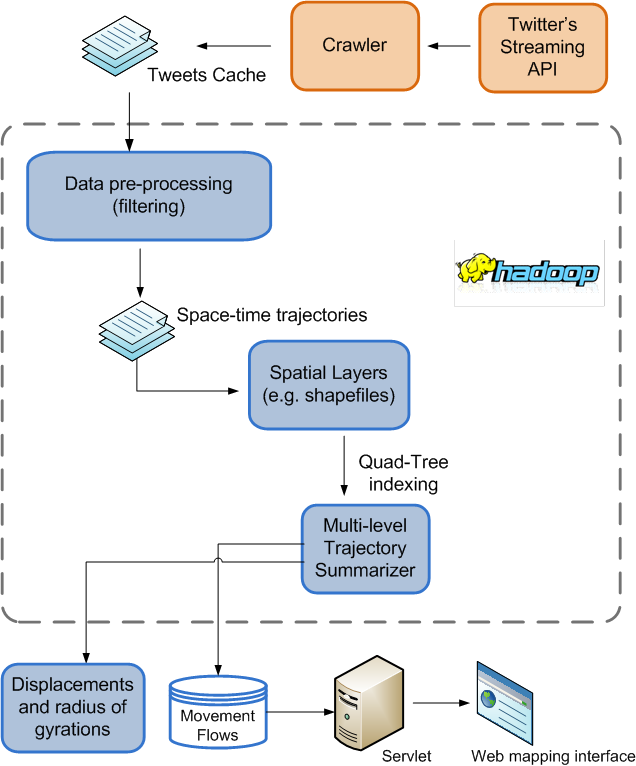
\includegraphics[width=0.6\linewidth]{./figures/Overall_Architecture222}
\caption{The overall system architecture of the framework}
\label{fig:Arch}
\end{figure}
%\FloatBarrier

\subsection{Space-time Twitter user trajectories}
To derive meaningful mobility patterns of individuals, a space-time trajectory of each individual user should be constructed~\citep{hagerstrand1985time}.
Each raw geo-located tweet contains multiple fields of information, such as the created time, country, language code, and location, etc. To construct a space-time trajectory from the data collection, we are interested in the following fields: \textit{User ID, location, timestamp}, which can be represented by a tuple $\left\langle id, loc, t\right\rangle$, where \textit{id} is a unique string representing a Twitter user's id; \textit{loc} is the recorded location of the message represented as a pair of projected coordinates $\left\langle x, y\right\rangle$;
and \textit{t} is the timestamp of when the message was posted; A Twitter user's space-time trajectory is defined as follows.
\newline

\noindent\emph{\textbf{Definition 1. Space-time Twitter user trajectory:}} The space-time trajectory of a Twitter user is defined as a collection of recorded geo-locations in the chronological order (i.e., based on the attached timestamp):
\newline

$Trajectory_{user_{id}} \equiv \lbrace \langle id, loc_{1}, t_{1}\rangle, \langle id, loc_{2}, t_{2}\rangle, \langle id, loc_{i}, t_{i}\rangle, ... \langle id, loc_{n}, t_{n}\rangle \rbrace, i = 1, 2, 3...n$
\newline

To remove non-human users based on unusual relocating speed, a user will be removed if the speed between any two consecutive locations in the user's trajectory with $speed$ $(loc_{i} - loc_{i-1}) > 240 m/s $.
\newline

\noindent\emph{\textbf{Definition 2. visitation behavior, displacement and radius of gyration:}} As each space-time Twitter user trajectory records all the locations a user has visited, the visitation behavior refers the frequency of a user visiting different locations within a specific time frame.
This metric can provide an overall assessments regarding the diversity and similarity in the collective mobility pattern~\citep{gao2012exploring}.

In particular, the measurements of displacements and radius of gyrations of individuals are two popular metrics to investigate and quantify the distance decay effects in the collective mobility patterns~\citep{gonzalez2008understanding}.
The displacement refers to an individual's re-allocation in the geographical space measured in distance, i.e., $distance (loc_{i} - loc_{i-1})$. It is not equivalent to a ``trip" took by an individual, for example, even the time interval between two recorded locations is one month, it will still count as a displacement.  
By studying all the displacements from a group people, it helps to identify the distance bounds associated with different travel modes~\citep{Jurdak2015} or to determine whether movements are random walks~\citep{brockmann2006scaling}.
Radius of gyration is a metric to distinguish mobility patterns of individuals~\citep{gonzalez2008understanding}, which is defined as fellows.   
\newline

$r_{g} = \sqrt{\frac{1}{n}\sum_{i=1}^{n}(p_{i} -  p_{centroid})^{2}}$, where $p_{centroid} = \frac{1}{n}\sum_{i=1}^{n}p_{i}$
\newline

\noindent It measures the accumulated distances of deviation from the center of mass of an individual user's trajectory, where $p_{i}$ is one of the user's locations and $p_{centroid}$ is the center of mass of the user's trajectory. When applying the measurements to all the users, it helps to identify different groups of people and understand the corresponding mobility patterns. Note that both displacements and radius of gyrations are measured by ``crow's fly distance" in this study (i.e., the direct distance between two recorded locations).
Since all these metrics are based on the generated trajectories, by breaking and aggregating the trajectories in multiple spatial scales and temporal granularity, it would enable performing multi-level spatiotemporal analysis of these measurements and studying the corresponding mobility patterns. 

\subsection{Multi-level spatiotemporal trajectory aggregation}
An important strategy for visual-analytics methods dealing with massive movement datasets is performing spatial aggregations to provide different levels-of-detail~\citep{andrienko2007designing,andrienko2007visual}.
It is similar to the map generation approach that when a user is interacting with a map interface, the details of visualization should be adaptive to a user's area-of-interest~\citep{buttenfield1991map}.
To enable aggregating Twitter trajectories into multiple spatial levels, we have extended the hierarchical space-time cube model developed in~\citep{cao2014scalable}, where we partitioned the geographic space of the United States into 10 hierarchical spatial layers. 
To be specific, the state boundaries of the United States are treated as the base layer (i.e. level 0) for aggregating state-level Twitter user movements, Alaska and Hawaii are excluded for the consideration of better visualization effects in the mapping interface of the framework. We then created an hierarchical fishnet by diving the study region into regular cells, where the finest level (level 10) consists 1km $\times$ 1km cells. Such a cell size is consistent with the spatial resolution in landscan\footnote{http://web.ornl.gov/sci/landscan/} product for measuring the global population density. In our case, the cell size for level i-1 is twice of the size in level i. Figure 2 illustrates an hierarchical fishnet spatial units for mapping multi-level Twitter user movements. Note that any fine-grained geographic boundaries can be used and appended in this framework to show different level-of-detailed movements (e.g., county-level and census-tract level), in our case, we replaced the level 8 fishnet layer with the US county boundaries.   

To perform a multi-level spatial aggregation of the Twitter user trajectories using hierarchical spatial layers, each location in a user's trajectory is redistributed to the corresponding spatial units. A MapReduce algorithm for the spatial aggregation is implemented, where the ID of unit in each spatial layer (e.g., polygon in state and country layer and cell in the rest) is treated as key in the at the map stage. It performs a ``point-in-polygon" process to determine which polygon the point belongs to. If the location does not belong to any polygon, it will be dropped, which is how we used the geographic boundaries of the United States to filer the raw tweet collection and keep the ``domestic" ones. To optimize the ``point-in-polygon" determination without comparing the location with every polygon in the spatial layer, we also created a Quad-Tree~\citep{samet1984quadtree} for each spatial layer to speed up the process. Finally, the reducers generate two data outputs: (1) reconstructed space-time Twitter user trajectories at each spatial level (2) movement flows in the form of in and out volumes among the units. The movement flows are stored in the database for interactive explorations in the web mapping interface, whereas the re-constructed trajectories can be further processed to produce distance measures at different spatial scales, which is illustrated as fellows:
\newline

\noindent $Trajectory_{user_{id}} \equiv \lbrace \langle id, loc_{1}, t_{1}, unit_{1}\rangle, \langle id, loc_{2}, t_{2}, unit_{2}\rangle, \langle id, loc_{i}, t_{i}, unit_{i}\rangle, ... \langle id, loc_{n}, t_{n}, unit_{n}\rangle \rbrace$
where $ i = 1, 2, 3...n$

\begin{figure}[h]
\centering
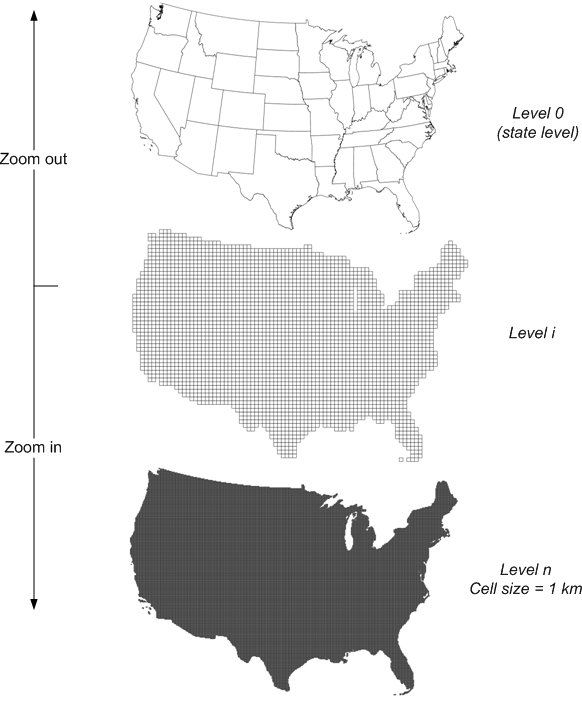
\includegraphics[width=0.6\linewidth]{./figures/multilevel}
\caption{Hierarchical spatial layers for aggregating movements in different level-of-details}
\label{fig:multilevel}
\end{figure}
%\FloatBarrier

\section{Multi-scale spatiotemporal Twitter user mobility patterns}
\subsection{Spatiotemporal Twitter user mobility patterns}
The situation of using geo-located tweets to track people's movements is complex as users' tweeting behavior can be significantly different from one to another, in particular the frequency and time-interval between two consecutive tweets. For example, some people may tweet once a day while others do more; some people may tweet regularly while others do not.  
These tweeting behaviors are expected as such human dynamics are also seen in the mobile phone call data~\citep{gonzalez2008understanding}. 
Many studies have carried out data collection within a certain time period (e.g., a year in our case).
However, as the geo-located tweets were collected in a continuous fashion, we need to examine the sensitivities regarding these behaviors to make sure we are not just capturing a random snapshot from the whole data streams. 

In this study, we have analyzed the cumulative distribution of the frequency Twitter users visiting different locations in year 2014 (and every month), which uses the methods developed in~\citep{clauset2009power}. 
The frequency is summarized based on the trajectories of individuals extracted in each time range. Note that different groups of Twitter user may exist in each month. 
It appears that the distribution of the collective Twitter user visitation behaviors in year 2014 follows a two-tiered power law distributions (shown in Figure 4), where the majority (the front part) of the distribution follows a truncated power-law distribution $p(x)\sim x^{-\alpha}e^{-\lambda x}$ and the $\alpha$ value is 1.32, and the tail part (less than 2$\%$ of the whole population) follows a power-law distribution  $p(x)\sim x^{-\alpha}$ with $\alpha$ value is 3.5.
This finding is consistent across all 12 months, with the mean $\alpha$ value as 1.34 $ \pm$  0.05 (standard deviation) and the mean $\lambda$ value as 0.00178 $ \pm$  0.0002 (standard deviation). 

The two-tier power law distribution indicates that the collective behaviors of Twitter user visiting different locations can be well approximated with a (truncated) L\'{e}vy Walk model~\citep{ reynolds2012truncated, rhee2011levy}, which has also been identified in many human mobility studies using different mobility data~\citep{zhao2015explaining}.
The similarities among the cumulative distributions suggest that the mobility data collected from geo-located tweets are temporally stable, at least at the monthly interval, which indicates studies collected geo-located tweets in one month can potentially reveal similar findings as the ones collected in multiple months. 
Of course, different spatial scales can effect such findings as we learned that there were no geo-located tweets collected from 4 counties.
In addition, the two-tier power law also reveals the diversity in the Twitter user visiting behaviors: (1) a small group Twitter users visited significantly more locations than the rest (2) within each group, the probability of Twitter user visiting more locations decreases significantly with a power function.

\begin{figure}[h]
\centering
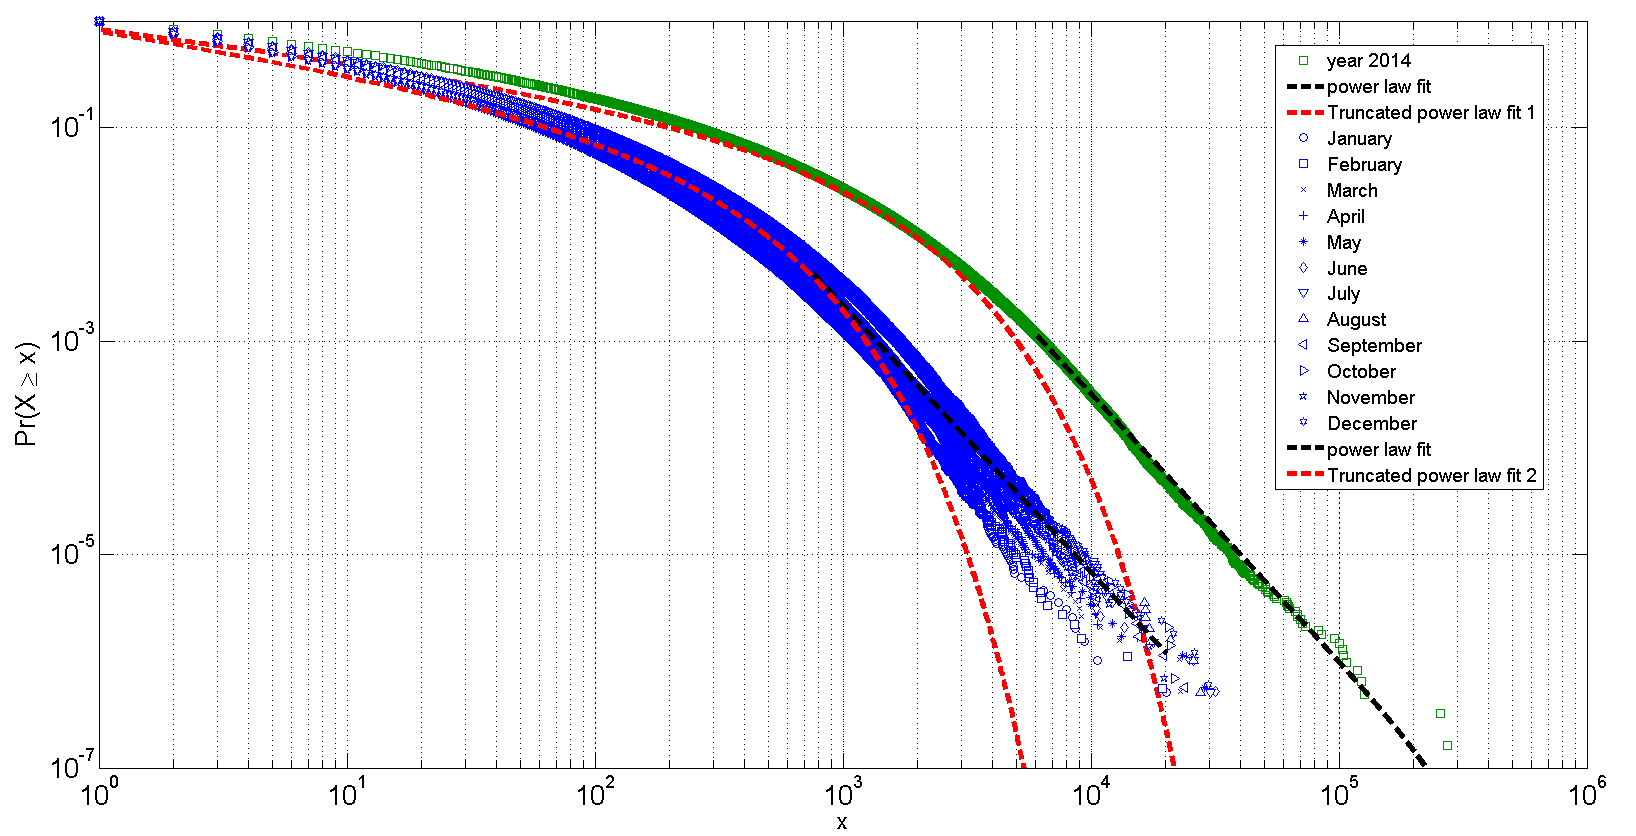
\includegraphics[width=1.0\linewidth]{./figures/visitation2}
\caption{Two-tier power law distribution of the collective Twitter user visitation behaviors}
\label{fig:Arch}
\end{figure}
%\FloatBarrier

As it is mentioned earlier, the measurements of displacements and radius of gyrations of individuals are two popular metrics to investigate and quantify the distance decay effects in the collective mobility patterns~\citep{gonzalez2008understanding}. In this case, we first gathered the displacements from all the collected Twitter users in the United States (excluding Hawaii and Alaska) in year 2014, where those Twitter users with only one geo-located tweet were filtered out. 
In addition, to investigate the mobility patterns of individuals, we derived the accumulated displacements and the radius of gyrations of each individual Twitter user based on the corresponding space-time trajectories over the one year period.
Note that both displacements and radius of gyrations were measured by ``crow's fly distance", which is the direct distance ($d$) between two consecutively recorded locations in a user's trajectory.

To seek mobility patterns from these measurements, we performed statistical analysis regarding the probability distributions of displacements and radius of gyrations, which is also known as the spatial dispersal kernel $P(d)$~\citep{brockmann2006scaling}. The probability distribution of the user displacements (as well as accumulated displacements) is shown in Figure 5, whereas the probability distribution of radius of gyrations is shown in Figure 6. In this study, we used the fitting methods developed by~\citep{Jurdak2015}. The probability distributions of overall displacements, and the accumulated displacements and radius of gyrations of individuals, can all be approximated by a combination of three functions: an exponential function, a stretched-exponential function and a power-law function.

In particular, as it is shown in Figure 5 (a), the probability distributions of overall displacements is approximated by $P(d) \sim \lambda_{1} e^{-\lambda_{1}(d - d_{min})}, d_{min}=10m$ from [10 m, 70m] (accounting for 2 $\%$ of the population),  $ P(d) \sim \beta\lambda_{1}d^{\beta-1}e^{-\lambda^{1}(d^\beta-d_{min}^\beta)}, d_{min} = 100m$ from [100m, 80km] (accounting for 93 $\%$ of the population), and $P(d) \sim {d}^{-\alpha}$ [$>$ 80km] (accounting for 5 $\%$ of the population). In additon, the displacement in the distance bound from 100m and 80km in Figure 5 (b) can be further approximately by two power-law distributions with a cutting point at 5km (53$\%$ distances are less than 5km and 40$\%$ distances between 5km and 80km), which indicates two different travel modes, such as inter- or intra-city movements.
Overall, the fitting functions with different distance bound suggest the existence of multi-scale or multi-modal mobility patterns ~\citep{Jurdak2015} of the Twitter users in the United States, for example the displacements larger than 80km could be related to inter-state travels or travel by flight. 

The probability distribution of radius of gyrations of individuals (Figure 6 (a)) is approximated by $P(r_{g}) \sim \lambda_{2} e^{-\lambda_{2}(r_{g} - {r_{g}}_{min})}, {r_{g}}_{min}=10m$ from [10 m, 50m], $P(r_{g}) \sim \lambda_{2} e^{-\lambda_{2}(r_{g} - {r_{g}}_{min})}$ from [50m, 30km], and $P(r_{g}) \sim {r_{g}}^{-\alpha}$ [$>$ 30km]. In particular, the radius of gyration between 50m and 30km can be further approximately by two power law distributions with a cutting point at 6km, which suggest two main types of spatial coverage of from the collected Twitter users in the United States. The distribution shows that around $10\%$ the tweet population has a radius of gyration less than 50 meters, which indicates those twitter users mostly tweet at a particular place, such as home or office;  around 60$\%$ of the population has a radius of gyration less than 30 km, which indicates that most of the collected Twitter user movements are ``short" distances, e.g., within a city locale. Note that the accuracy of these values for defining the distance bound depends on the accuracy of the location information of each geo-located tweet. 

\begin{figure}[h]
\centering
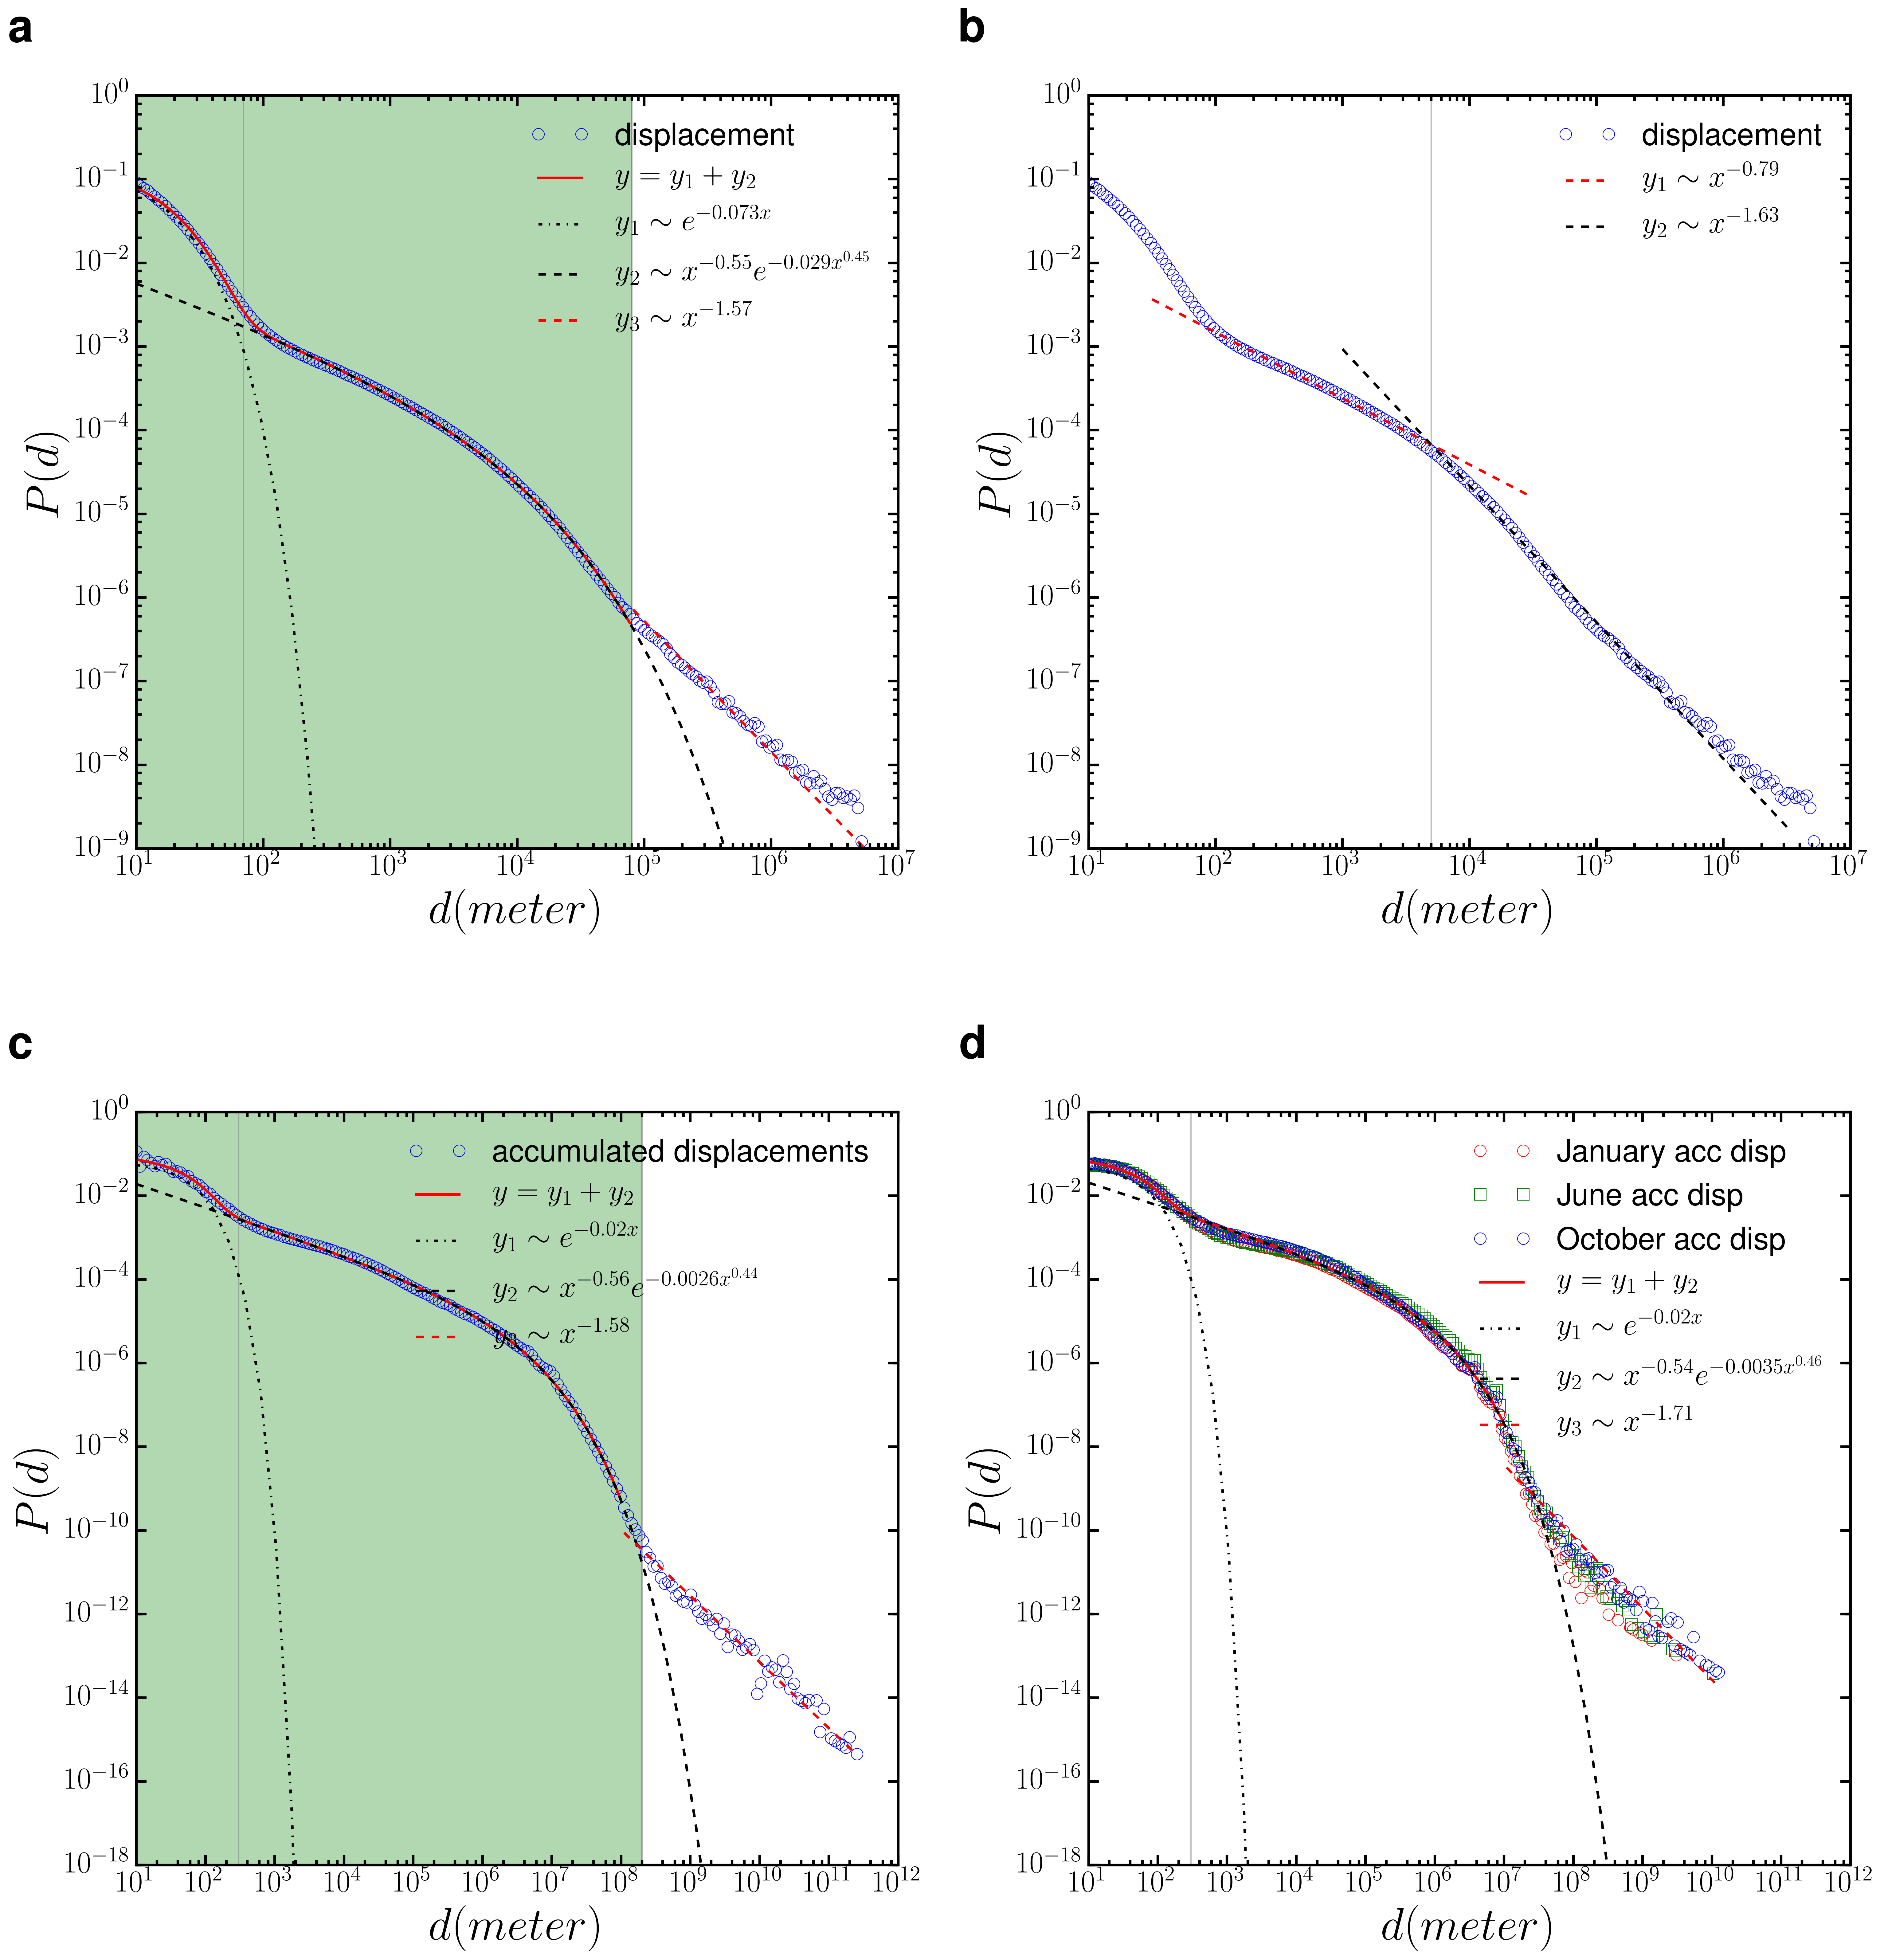
\includegraphics[width=1.0\linewidth]{./figures/displacement}
\caption{(a) The probability distribution of the collective Twitter user displacements P(d) (b) the distance between [100m, 80km] is approximated by a double power-law functions (c) The probability distribution of the accumulated displacements of individual Twitter users P(d) (d) The probability distribution of the accumulated displacements of individual Twitter users in 3 different months}
\label{fig:Arch}
\end{figure}\textbf{}
%\FloatBarrier

\begin{figure}[h]
\centering
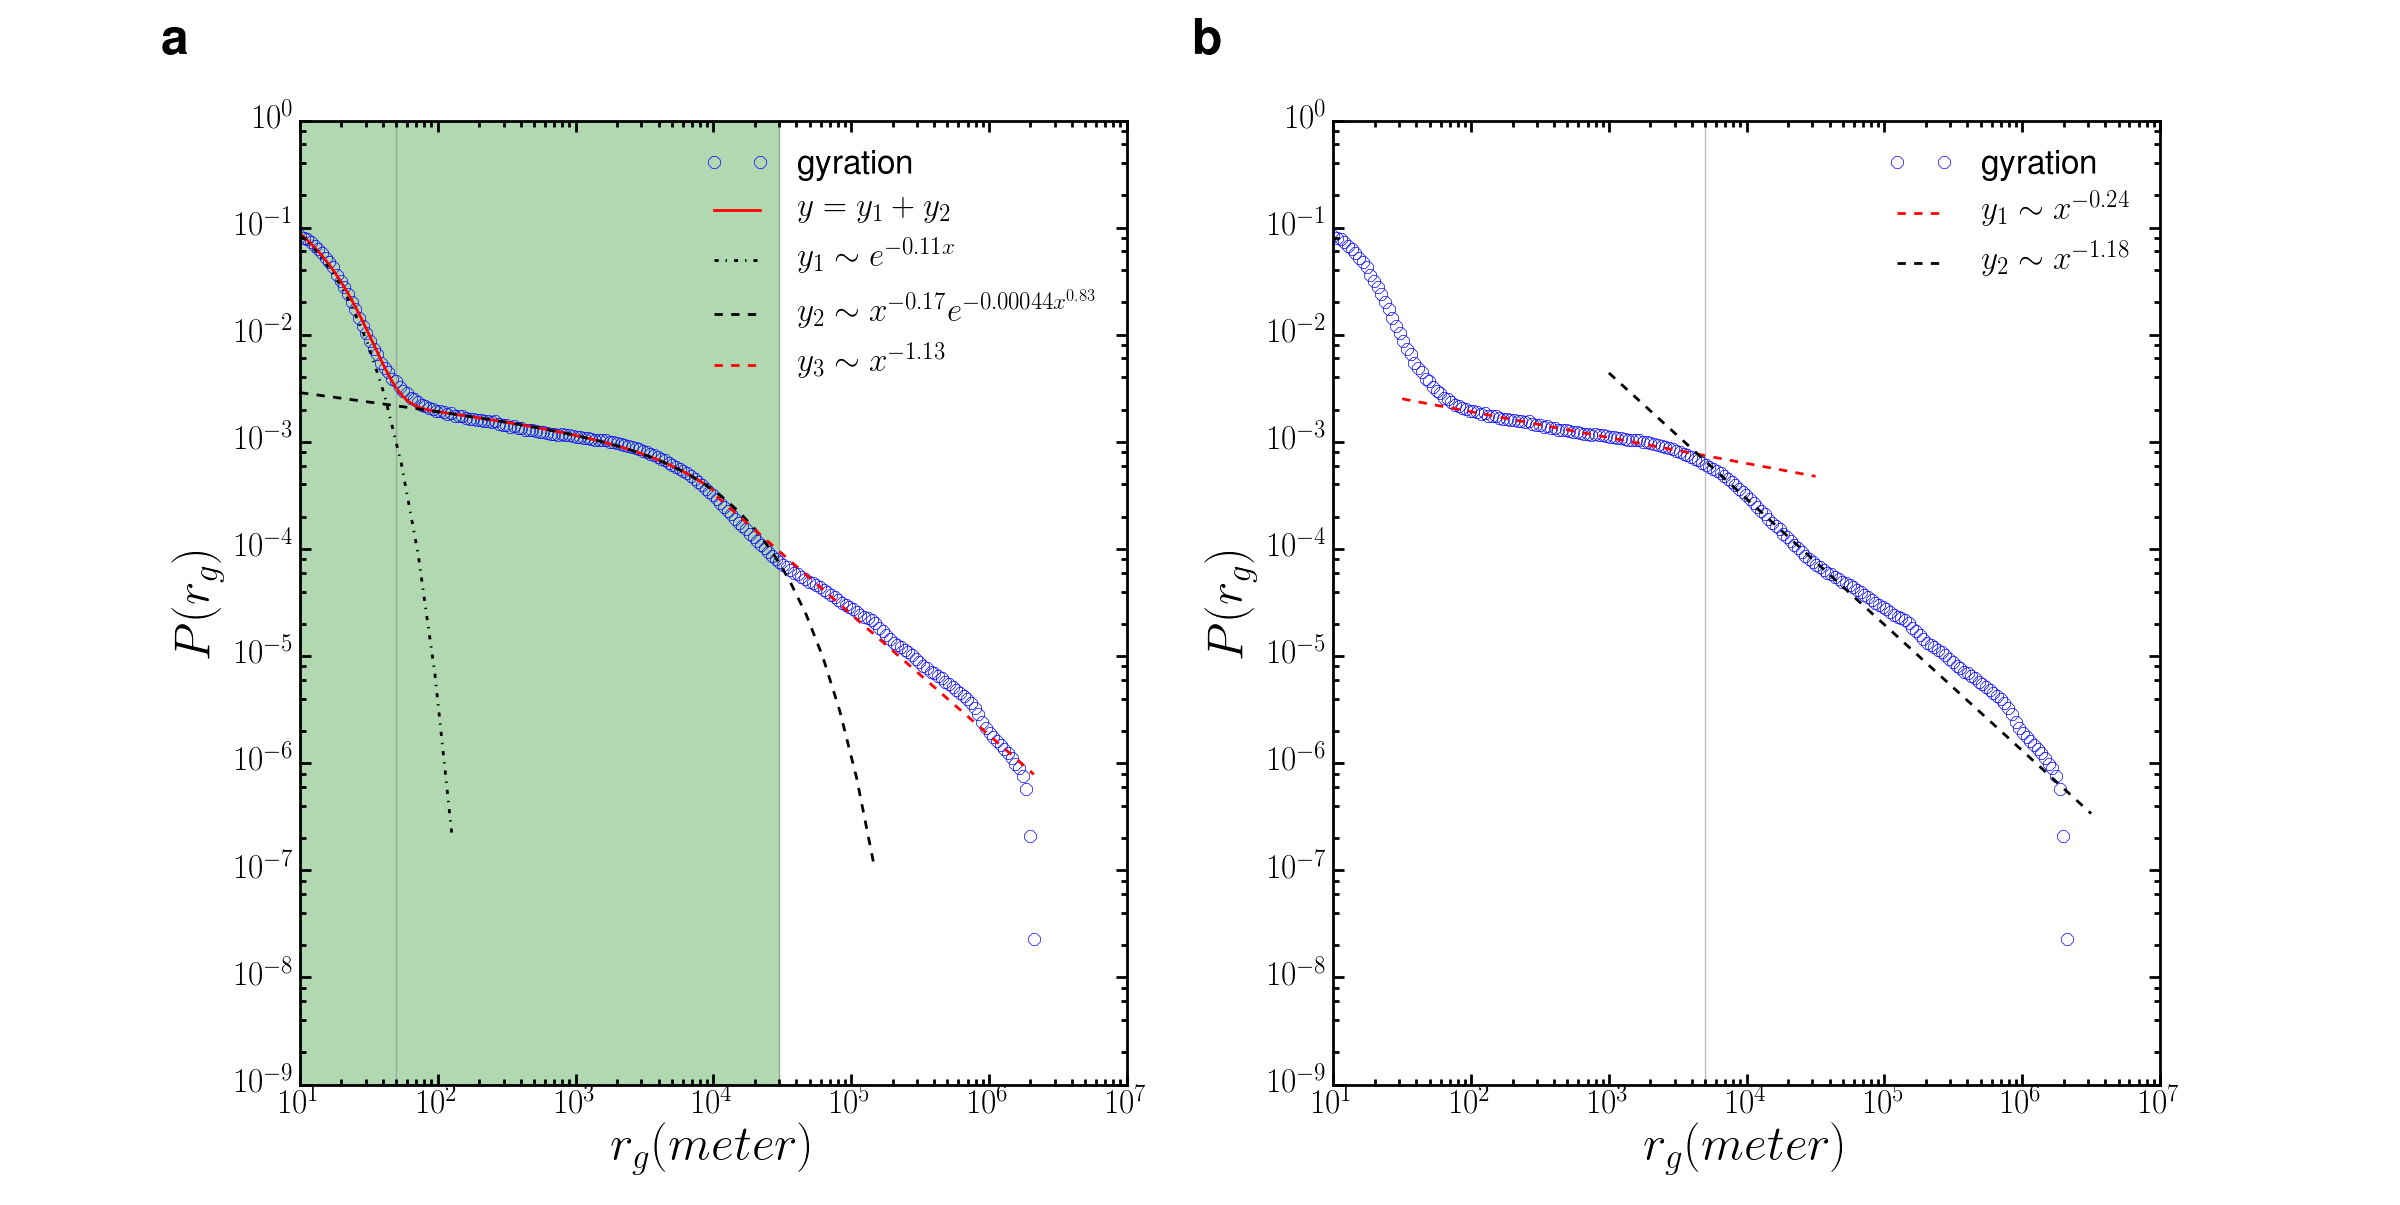
\includegraphics[width=1.0\linewidth]{./figures/gyration}
\caption{ (a) The probability distribution of radius of gyration of individual Twitter users P($r_{g}$) (b) the distance between [50m, 30 km] is approximated by a double power-law functions}
\label{fig:Arch}
\end{figure}
%\FloatBarrier

More importantly, as our framework can aggregate Twitter user trajectories within different temporal ranges, we further analyzed the probability distributions of accumulated displacements took places in January, June, and October (Figure 5 (d)) and radius of gyrations within 4 quarters in year 2014 (Figure 7), in order to examine whether there are temporal changes in the mobility patterns. While the probability distributions of accumulated displacements are almost identical in those selected three months,  we do find changes in the probability distributions of radius of gyrations in different quarters of the year. 
The fluctuations in the tails of the distributions indicate that long distance radius of gyrations (i.e., above 30 km) will experience more seasonal changes in the Twitter user mobility pattern, which means the increase or decrease of long distance movement activities in the corresponding time period. 
However, it is worthy noting that the overall trends in the Twitter user mobility patterns revealed by radius of gyrations are still consistent.  In summary, by comparing these results with the same measurements in~\citep{Jurdak2015}, (slightly) different distance bounds were identified for describing the Twitter user mobility patterns in the USA and Australia, however the overall similarity and consistence found in using a combination of three functions to approximate the probability distribution functions of displacements and radius of gyrations, clearly provide supports for using geo-located tweets for conducting replicable human mobility studies.       
 
\begin{figure}[h]
\centering
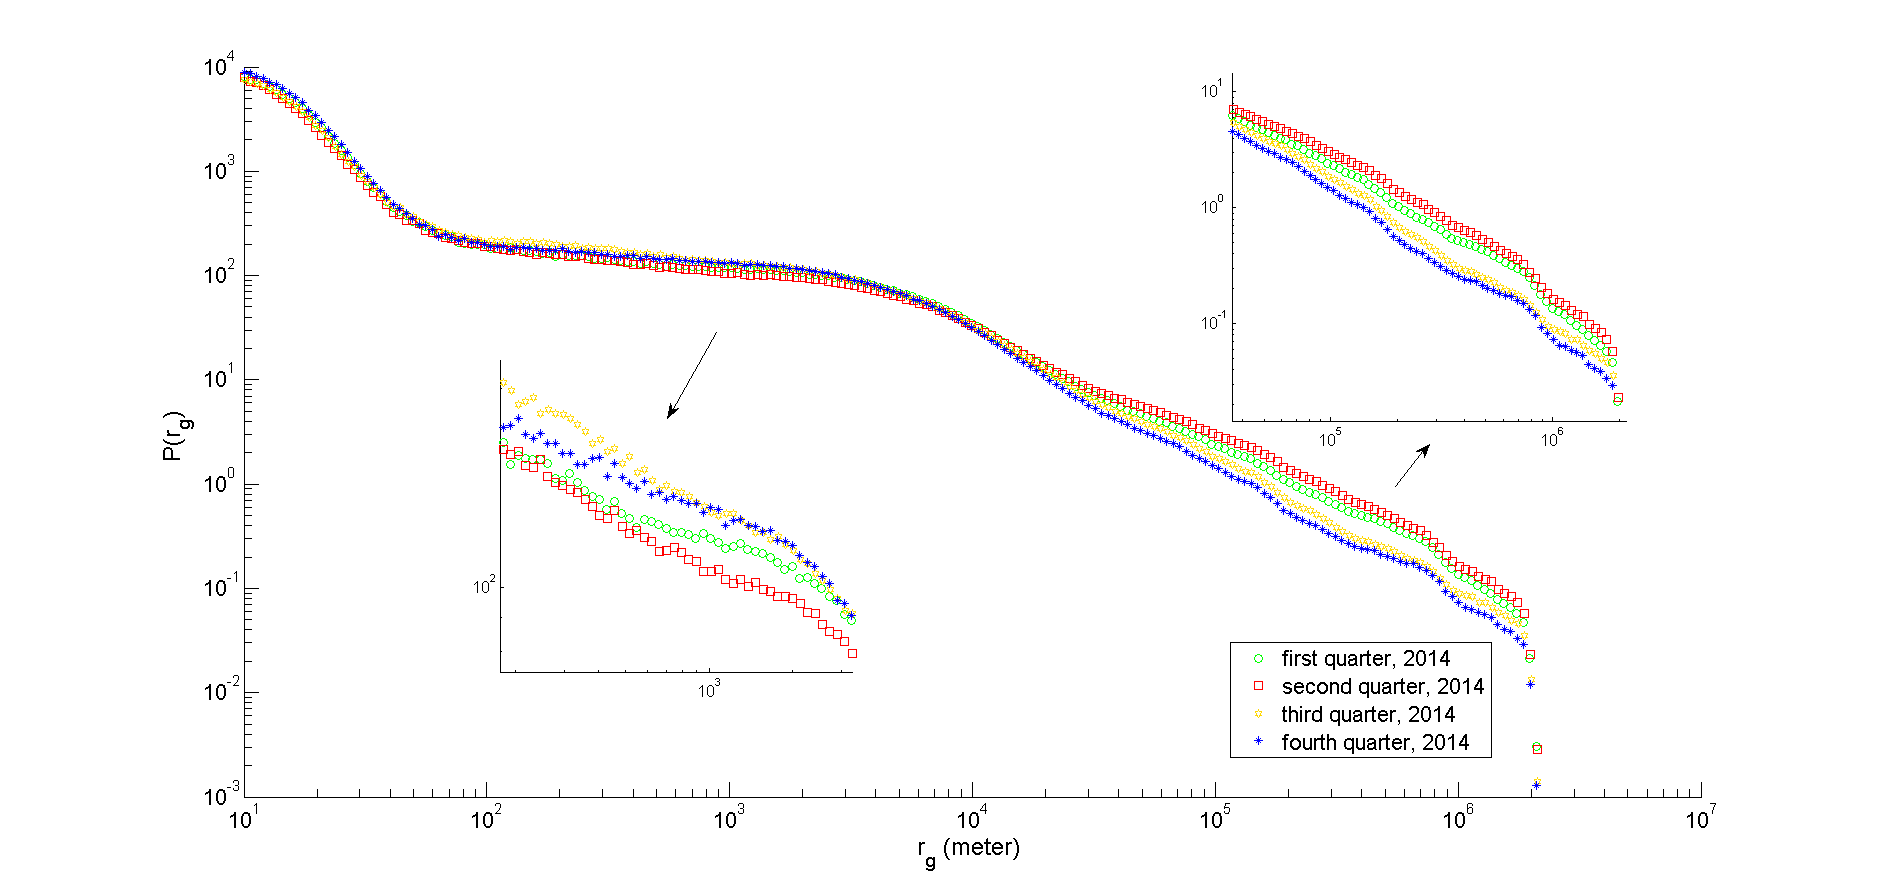
\includegraphics[width=1.0\linewidth]{./figures/gyration_season}
\caption{The probability distribution of radius of gyration of individual Twitter users in different quarters of year 2014}
\label{fig:Arch}
\end{figure}
%\FloatBarrier

The above analysis of Twitter user mobility patterns mainly focus on the temporal aspects where the spatial scale is fixed to the country level.
Our framework provides the flexibility to aggregate and extract Twitter user trajectories in a specific spatial scale and re-produce the analysis. 
In particular, as it is evident from the above analysis that there are multi-scale or multi-modal Twitter user mobility patterns, this framework can help further look into the mobility pattern regarding how Twitter users move across different spatial scales and temporal ranges, which is measured by the movement flows among these spatial regions.  In this case, we demonstrate the inter-state mobility patterns by using the framework to capture the movement flows among the states. Note that the movement flows can be summarized across all the 10 spatial layers in the framework. 
In particular, the movement flows in the state level are summarized and visualized with chord diagrams (illustrated in Figure 10) as part of the interactive mapping interface.
We tested the overall distribution of the movement flows (in the form of weighted in-degree and out-degree of a graph, where each state is treated as a node) among different states in year 2014.  
We found that the probability distribution of Twitter user movement flows of visiting different states follows a log-normal distribution: $p(x)\sim \frac{1}{x}exp[-\frac{(lnx - \mu)^{2}}{2\sigma^{2}}]$, which suggests the flux of Twitter user movements among the states are highly skewed and dominated by a few states. It also indicates that although the Twitter population seems to be linearly correlated with the population at state level, it is not proportional to account the movement flux among the states, which may provide some insights for other researchers in studying social-economical aspects of the migration dynamics.

\begin{figure}[h]
\centering
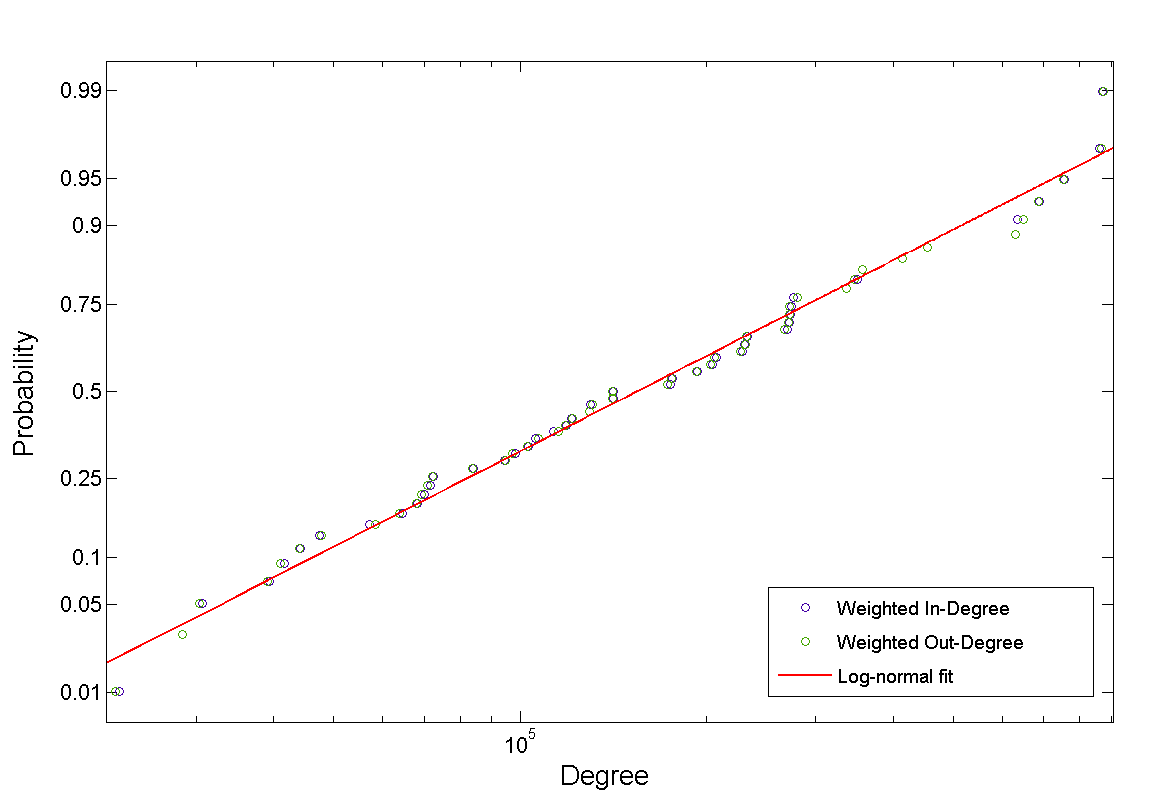
\includegraphics[width=0.8\linewidth]{./figures/degree}
\caption{The distribution of Twitter user movement flows among different states in year 2014 measured in weighted in- and out-degrees}
\label{fig:Arch}
\end{figure}
%\FloatBarrier

\subsection{The interactive 3D virtual globe web mapping interface}
In addition to providing supports for understanding Twitter user mobility patterns with statistical analysis, the framework integrates a 3D virtual globe interface to enable users to perform exploratory geo-visual analytics of the multi-level spatiotemporal Twitter user movements. 
The 3D virtual globe is developed and extended from the Cesium library\footnote{http://cesiumjs.org/}, which is an open-source WebGL virtual globe and map engine. 
We customized the map engine to adapt different spatial scales, which correspond to the hierarchical spatial layers,  for aggregating movements in different level-of-details.
The map interface interprets user's interactions, such as area-of-interest, time window, and zoom levels, etc. as parameters and send to the dedicated visualization servlet on the CyberGIS Gateway\footnote{http://sandbox.cigi.illinois.edu/home/}, which is the leading online cyberGIS environment for a large number of users to perform computing- and data-intensive, and collaborative geospatial problem-solving enabled by advanced cyberinfrastructure~\citep{liu2014cybergis}.
In return, the map interface visualizes the corresponding movement flows on the virtual globe.

An overview of the web mapping interface is shown in Figure 8. In terms of performing exploratory visual-analytics of Twitter user movement patterns, users can specify the time window to enable the query. 
When the results are shown, users can hover the mouse over each individual lines on the map to see the value of movement flows for both in and out directions. If the selected criteria keep unchanged, whenever the user zooms in/out, tilt or rotate the globe, the mapping interface will automatically provide the corresponding level-of-details on the fly.

\begin{figure}[h]
\centering
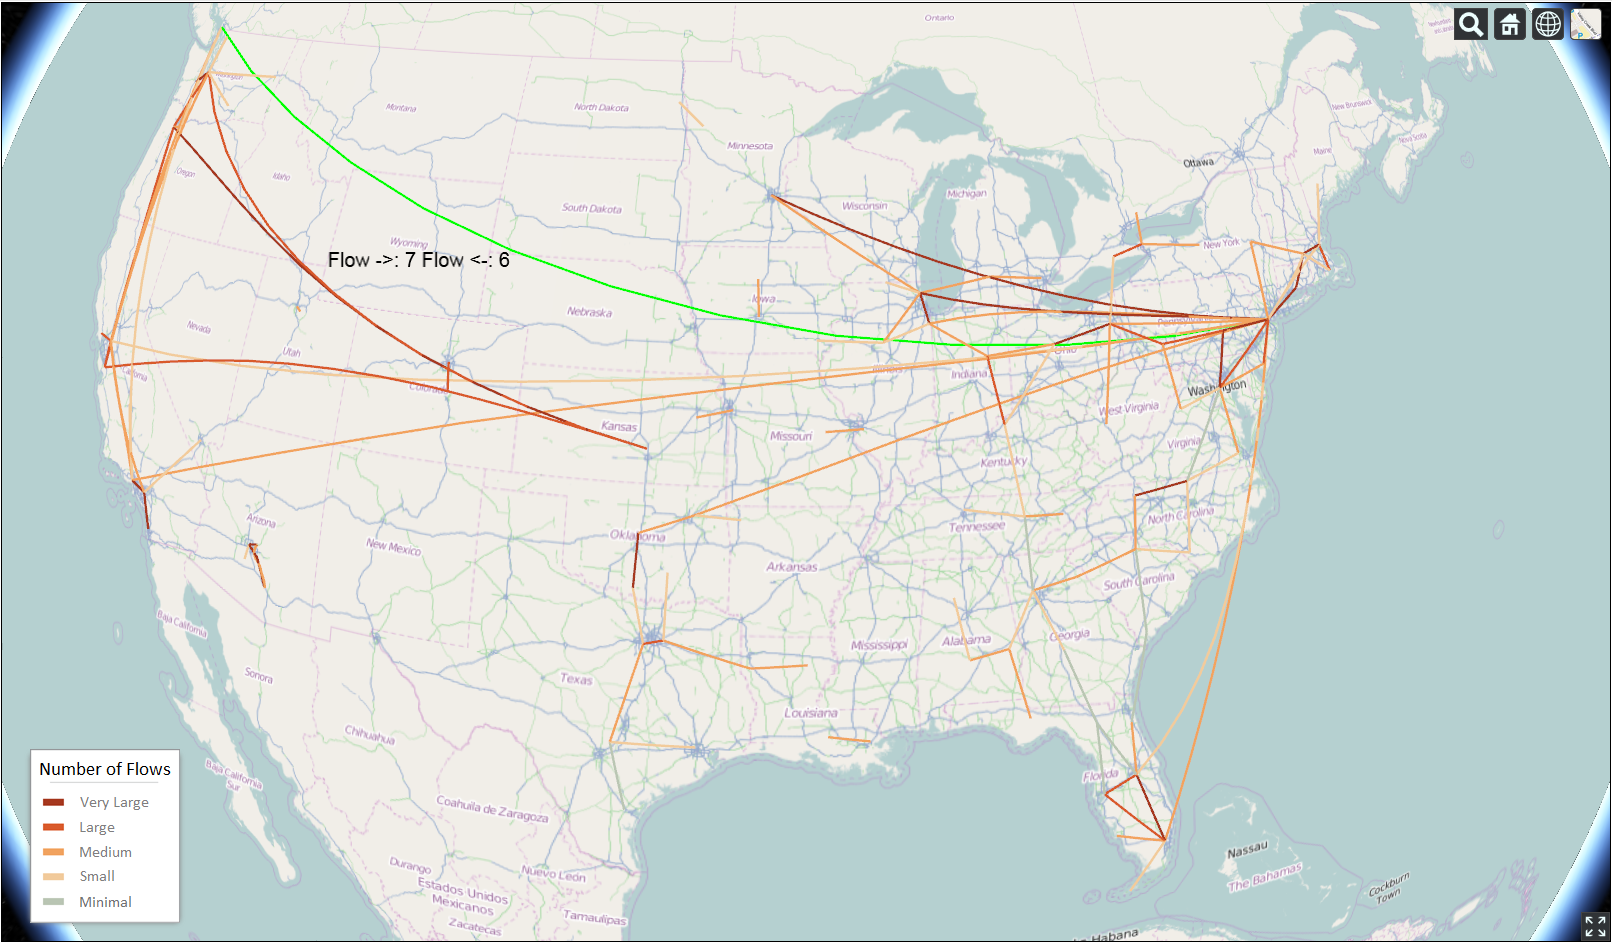
\includegraphics[width=0.8\linewidth]{./figures/vocation}
\caption{An overview of the 3D interactive web mapping interface}
\label{fig:Web_Interface}
\end{figure}
%\FloatBarrier

For state level Twitter user movements, we provide an interactive chord diagram to explicitly illustrate the movement flows among different states (Figure 9). Figure 9 demonstrates the Twitter movement flows among different states in January, 2014. The size of each color patch is proportional to the volume of total incoming movements from other states, which allow us to visually identify those states that dominate the incoming movement flows and which states the flows are generated from.
By interacting with the state names, it will highlight the details of incoming movement flows from other states, in this case California is selected, which has the largest incoming movement flows in January.\newline

\begin{figure}[h]
\centering
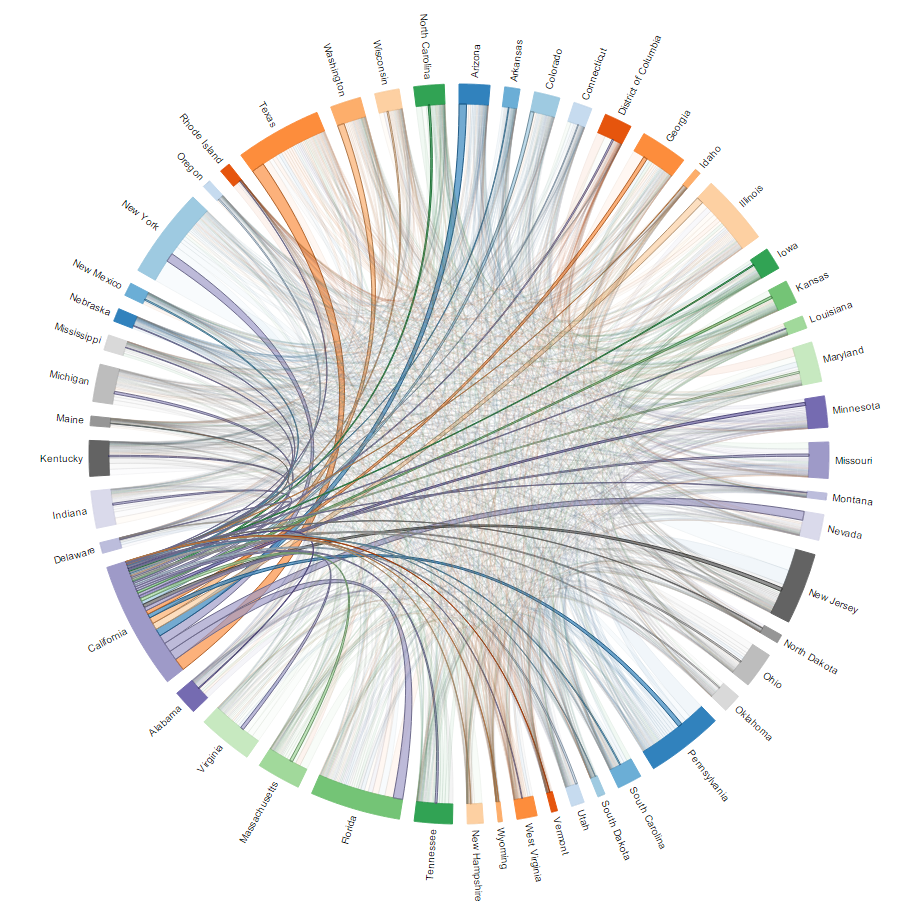
\includegraphics[width=1.0\linewidth]{./figures/vaca_flow}
\caption{Chord diagrams for the movement flows among different states in January, 2014}
\label{fig:vaca_movement}
\end{figure}
%\FloatBarrier


\section{Conclusions}
In this study, we have used large volume of geo-located tweets to study Twitter user mobility patterns across multi-level spatial scales and temporal granularity in the United States during the year 2014. 
To address the data-intensive challenges, we have developed a scalable visual-analytics framework tailored to accommodate large volume of geo-located tweets for studying multi-level spatiotemporal Twitter user mobility patterns.
This framework is implemented based on high-performance distributed computing environment using Apache Hadoop.
It delivers scalability in filtering large volume of geo-located tweets, modeling and extracting Twitter user movements, generating space-time user trajectories, and summarizing multi-level spatiotemporal user mobility patterns.

With this framework, we have found some interesting Twitter user mobility patterns, both statistically and visually.
We studied the collective Twitter user visiting behavior regarding the frequency of Twitter users visiting different locations, which was fitted by a two-tier power-law distribution function.
The two-tier power law distribution indicates that the collective behaviors of Twitter user visiting different locations can be well approximated with a (truncated) L\'{e}vy Walk model, which has also been identified in many human mobility studies using different mobility data.
The similarities among the cumulative distributions suggest that the mobility data collected from geo-located tweets are temporally stable, at least at the monthly interval, which provides supports that we are not just capturing a random snapshot of the whole data stream. 

We studied the distance decay effects in the collective Twitter user movements measured by the probability distributions of the displacements and radius of gyrations of individuals. 
These distributions can all be approximated by a combination of three functions: an exponential function, a stretched-exponential function and a power-law function. In particular, distance bounds between different fitting functions in displacement distribution reveals the existence of multi-scale or multi-modal mobility patterns of the Twitter users in the United States, whereas the distribution of radius of gyration reveals different groups of Tweet users with different types of spatial coverages.   
More importantly, we further studied these mobility patterns in different temporal scales to investigate the temporal changes in the mobility patterns. 
We found that the accumulated displacements are almost identical in different months, while the long distance radius of gyration (i.e., above 30 km) will experience more seasonal changes in the Twitter user mobility pattern.



%%%%%%%%%%%%%%%%%%%%%%%%%%%%%%%%%%%%%%%%%%
%% optional
\supplementary{The following are available online at www.mdpi.com/link, Figure S1: title, Table S1: title, Video S1: title.}

%%%%%%%%%%%%%%%%%%%%%%%%%%%%%%%%%%%%%%%%%%
\acknowledgments{All sources of funding of the study should be disclosed. Please clearly indicate grants that you have received in support of your research work. Clearly state if you received funds for covering the costs to publish in open access.}

%%%%%%%%%%%%%%%%%%%%%%%%%%%%%%%%%%%%%%%%%%
\authorcontributions{For research articles with several authors, a short paragraph specifying their individual contributions must be provided. The following statements should be used ``X.X. and Y.Y. conceived and designed the experiments; X.X. performed the experiments; X.X. and Y.Y. analyzed the data; W.W. contributed reagents/materials/analysis tools; Y.Y. wrote the paper.'' Authorship must be limited to those who have contributed substantially to the work reported.}

%%%%%%%%%%%%%%%%%%%%%%%%%%%%%%%%%%%%%%%%%%
\conflictofinterests{Declare conflicts of interest or state ``The authors declare no conflict of interest.'' Authors must identify and declare any personal circumstances or interest that may be perceived as inappropriately influencing the representation or interpretation of reported research results. Any role of the funding sponsors in the design of the study; in the collection, analyses or interpretation of data; in the writing of the manuscript, or in the decision to publish the results must be declared in this section. If there is no role, please state ``The founding sponsors had no role in the design of the study; in the collection, analyses, or interpretation of data; in the writing of the manuscript, and in the decision to publish the results''.} 

%%%%%%%%%%%%%%%%%%%%%%%%%%%%%%%%%%%%%%%%%%
\bibliographystyle{mdpi}
\bibliography{lite}
%%%%%%%%%%%%%%%%%%%%%%%%%%%%%%%%%%%%%%%%%%
\end{document}

